\section{Modelo de datos de Cassandra}
\label{cap:cassandra}

Cassandra guarda las escuchas como serie temporal y las métricas agregadas por fecha que consume el dashboard \citep{cassandra}. MongoDB conserva el documento original y Neo4j las relaciones; aquí está lo que se consulta por tiempo y en volumen. El código está en \code{databases/cassandra/}.

\subsection{Por qué este diseño}

Son 4\,855\,809 escuchas y el DAG puede seguir agregando lotes, así que la base tiene que aceptar escrituras masivas. Las consultas del dashboard se conocen de antemano y son siempre las mismas: actividad por día, ranking del mes, evolución de un artista e historial de un usuario. En Cassandra eso se resuelve con una tabla por consulta (diseño \emph{query-first}), de modo que cada lectura va directo a una sola partición sin importar cuántos datos haya. Dentro de la partición, la clave de clustering deja las filas ordenadas por fecha. El costo es repetir datos entre tablas y no poder hacer consultas ad hoc: si aparece una pregunta nueva, hay que agregar otra tabla.

\subsection{Tablas}

El keyspace \code{music_dna} usa \code{SimpleStrategy} con factor de replicación 1, porque en desarrollo corremos un solo nodo. La tabla~\ref{tab:cassandra-tablas} resume las seis tablas.

\begin{table}[H]
\centering
\caption{Tablas del keyspace \code{music_dna}}
\label{tab:cassandra-tablas}
\small
\begin{tabularx}{\textwidth}{>{\raggedright\arraybackslash}p{3.3cm} >{\raggedright\arraybackslash}p{2.7cm} >{\raggedright\arraybackslash}p{3.2cm} Y}
\toprule
Tabla & Partición & Clustering & Consulta que responde \\
\midrule
\code{listens_by_user} & \code{(user_id, month)} & \code{listened_at DESC, listen_id} & Historial de un usuario en un mes \\
\code{daily_stats} & \code{year} & \code{day} & Serie diaria del año con sus KPIs \\
\code{top_artists_by_month} & \code{month} & \code{rank} & Top de artistas del mes, ya ordenado \\
\code{artist_monthly_listens} & \code{artist_name} & \code{month} & Evolución mensual de un artista \\
\code{user_daily_listens} & \code{user_id} & \code{day} & Actividad diaria de un usuario \\
\code{load_batches} & \code{batch_id} & -- & Lotes del archivo ya cargados \\
\bottomrule
\end{tabularx}
\end{table}

Las dos tablas principales se definen así en \code{schema.cql}:

\begin{lstlisting}[language=CQL]
CREATE TABLE IF NOT EXISTS music_dna.listens_by_user (
    user_id        bigint,
    month          text,
    listened_at    timestamp,
    listen_id      uuid,
    artist_name    text,
    track_name     text,
    release_name   text,
    recording_msid text,
    PRIMARY KEY ((user_id, month), listened_at, listen_id)
) WITH CLUSTERING ORDER BY (listened_at DESC, listen_id ASC);

CREATE TABLE IF NOT EXISTS music_dna.daily_stats (
    year             int,
    day              date,
    listens          bigint,
    active_users     int,
    listens_per_user double,
    growth_pct       double,
    PRIMARY KEY ((year), day)
);
\end{lstlisting}

Tres decisiones del modelo merecen explicación:

\begin{itemize}
  \item \code{listens_by_user} se particiona por usuario y mes, no solo por usuario. Así una partición no crece sin límite: la más grande del dataset tiene 14\,205 filas. Particionar solo por usuario habría acumulado todo el historial de los usuarios más activos en una sola partición.
  \item \code{top_artists_by_month} usa \code{rank} como clustering porque Cassandra solo ordena por columnas de clustering. El ranking se calcula al cargar y la consulta es un \texttt{SELECT ... LIMIT 10}.
  \item No se guarda \code{user_name}: con \code{user_id} alcanza y el dashboard no necesita exponer nombres de usuario.
\end{itemize}

\code{listen_id} es un UUID determinista (UUID versión 5) calculado a partir del usuario, el \code{timestamp}, el \code{recording_msid}, el artista y la canción. La misma escucha siempre genera el mismo id, y eso es lo que hace que recargar no duplique filas.

\subsection{Carga por lotes}

\code{databases/cassandra/loader.py} lee el JSONL en lotes de 500\,000 líneas. Para cada lote:

\begin{enumerate}
  \item Limpia cada línea: \code{user_id} y \code{timestamp} enteros, artista y canción no vacíos. Las líneas que no cumplen se cuentan como omitidas, y las escuchas repetidas dentro del lote (mismo \code{listen_id}) se descartan.
  \item Si el lote no está registrado en \code{load_batches}, escribe sus escuchas en \code{listens_by_user} y lo registra con sus conteos. El id del lote es el nombre del archivo más el rango de líneas, por ejemplo \code{listens_full.jsonl:1-500000}.
  \item Al terminar, recalcula las tablas agregadas (\code{daily_stats}, \code{top_artists_by_month}, \code{artist_monthly_listens} y \code{user_daily_listens}) con todas las escuchas cargadas hasta ese momento y las sobrescribe.
\end{enumerate}

Repetir la carga no duplica nada: las escuchas tienen id determinista y el \texttt{INSERT} sobrescribe la misma fila, los lotes registrados no se vuelven a escribir y los agregados se reemplazan en lugar de sumarse. La función \code{load_listens} acepta un máximo de lotes nuevos por ejecución, y eso es lo que usa Airflow para cargar un lote por corrida (sección~\ref{cap:airflow}). El tamaño de lote debe ser siempre el mismo, porque el id de cada lote depende de él.

Hicieron falta tres optimizaciones:

\begin{itemize}
  \item \textbf{BATCH por partición.} Las filas de la misma partición se envían juntas en un \texttt{UNLOGGED BATCH} de hasta 30 filas, que Cassandra aplica como una sola mutación. Fue unas 13 veces más rápido que una escritura por fila. Mezclar particiones en un mismo BATCH habría sido más lento.
  \item \textbf{Sin counters.} La primera versión usaba columnas \code{counter}, pero cada incremento lee antes de escribir, y con alrededor de un millón de claves artista--mes la carga se volvía cada vez más lenta. Además, si un reintento repite un lote, un counter suma dos veces. Recalcular y sobrescribir resultó más rápido y seguro.
  \item \textbf{\code{UNSET_VALUE} en lugar de \code{None}} para los campos opcionales, porque insertar \code{None} crea un tombstone (marca de borrado) por cada fila.
\end{itemize}

\subsection{Resultados de la carga completa}

Las mediciones se hicieron en un notebook con Windows~11, 20~GB de RAM y Cassandra~5.0 en Docker (un nodo, heap de 2~GB), cargando el archivo completo del incremental 2746 con las tablas vacías.

\begin{table}[H]
\centering
\caption{Tiempos de carga en Cassandra}
\label{tab:cassandra-tiempos}
\begin{tabularx}{\textwidth}{l Y}
\toprule
Etapa & Tiempo \\
\midrule
10 lotes de escuchas (lectura, limpieza y escritura) & 343~s, entre 7\,500 y 21\,600 filas por segundo según el lote \\
Recálculo de las tablas agregadas & 196~s \\
Total & 553~s (unos 9 minutos) \\
Segunda ejecución sin lotes nuevos & 439~s; los totales no cambian (4\,855\,809) \\
\bottomrule
\end{tabularx}
\end{table}

La segunda ejecución demuestra que la carga es idempotente, pero también muestra el costo del diseño: cada ejecución relee el archivo para recalcular los agregados, así que tarda unos 7 minutos aunque no haya lotes nuevos. Para el DAG es aceptable; si hiciera falta bajarlo, habría que recalcular solo los días y meses que tocó el lote nuevo.

\begin{table}[H]
\centering
\caption{Filas resultantes por tabla}
\label{tab:cassandra-filas}
\begin{tabularx}{\textwidth}{l Y}
\toprule
Tabla & Filas \\
\midrule
\code{listens_by_user} & 4\,855\,809 en 30\,315 particiones (la mayor, 14\,205 filas) \\
\code{artist_monthly_listens} & 961\,898 \\
\code{user_daily_listens} & 113\,827 \\
\code{daily_stats} & 7\,575 días, del 2005-02-13 al 2026-10-27 \\
\code{top_artists_by_month} & Hasta 50 artistas por cada uno de los 260 meses \\
\bottomrule
\end{tabularx}
\end{table}

El total se comprobó de tres formas independientes: la suma de \code{load_batches}, la suma de \code{daily_stats} y un \texttt{COUNT(*)} partición por partición en \code{listens_by_user}. Las tres dan 4\,855\,809, igual que \code{scripts/validate_dataset.py}, sin líneas omitidas ni duplicadas.

\subsection{Operaciones CRUD}

El CRUD está en \code{databases/cassandra/crud.py} y trabaja sobre \code{listens_by_user}, donde una fila es una escucha. Como \code{month} se calcula a partir de \code{listened_at}, para ubicar una escucha basta con \code{user_id}, \code{listened_at} y \code{listen_id}.

\begin{table}[H]
\centering
\caption{Operaciones CRUD en Cassandra}
\label{tab:cassandra-crud}
\begin{tabularx}{\textwidth}{l l Y}
\toprule
Operación & Función & CQL \\
\midrule
Insertar & \code{insert_listen} & \texttt{INSERT INTO listens\_by\_user (...) VALUES (...)} \\
Consultar una & \code{get_listen} & \texttt{SELECT * ... WHERE} con la clave primaria completa \\
Consultar el mes & \code{get_user_listens} & \texttt{SELECT * ... WHERE user\_id = ? AND month = ? LIMIT ?} \\
Actualizar & \code{update_listen} & \texttt{UPDATE listens\_by\_user SET track\_name = ?, release\_name = ?} con la clave \\
Eliminar & \code{delete_listen} & \texttt{DELETE FROM listens\_by\_user} con la clave \\
\bottomrule
\end{tabularx}
\end{table}

Dos detalles de Cassandra explican el código. Primero, \texttt{INSERT} y \texttt{UPDATE} son \emph{upserts}: un \texttt{UPDATE} sobre una fila que no existe la crea. Por eso \code{update_listen} y \code{delete_listen} leen la fila antes y devuelven \texttt{False} si no existe. Segundo, no usamos \texttt{IF EXISTS}. Lo probamos y fallaba: esas escrituras (transacciones ligeras) usan el reloj del servidor y las normales el del cliente. Con Docker en Windows, el \texttt{UPDATE ... IF EXISTS} respondía que se había aplicado, pero quedaba con un timestamp anterior al del \texttt{INSERT} y Cassandra conservaba el valor viejo.

La demostración (\code{python -m databases.cassandra.crud --step}) usa el usuario $-1$, que no existe en ListenBrainz: inserta una escucha, la lee, la corrige, la borra y comprueba que ya no está. Termina con una lectura real de las últimas escuchas de un usuario del dataset. El CRUD no modifica las tablas agregadas, que se recalculan en cada carga. La figura~\ref{fig:cassandra-crud} muestra los cuatro primeros pasos ejecutados contra el keyspace que dejó Airflow.

\begin{figure}[H]
\caption{Demostración del CRUD en Cassandra}
\label{fig:cassandra-crud}
\centering
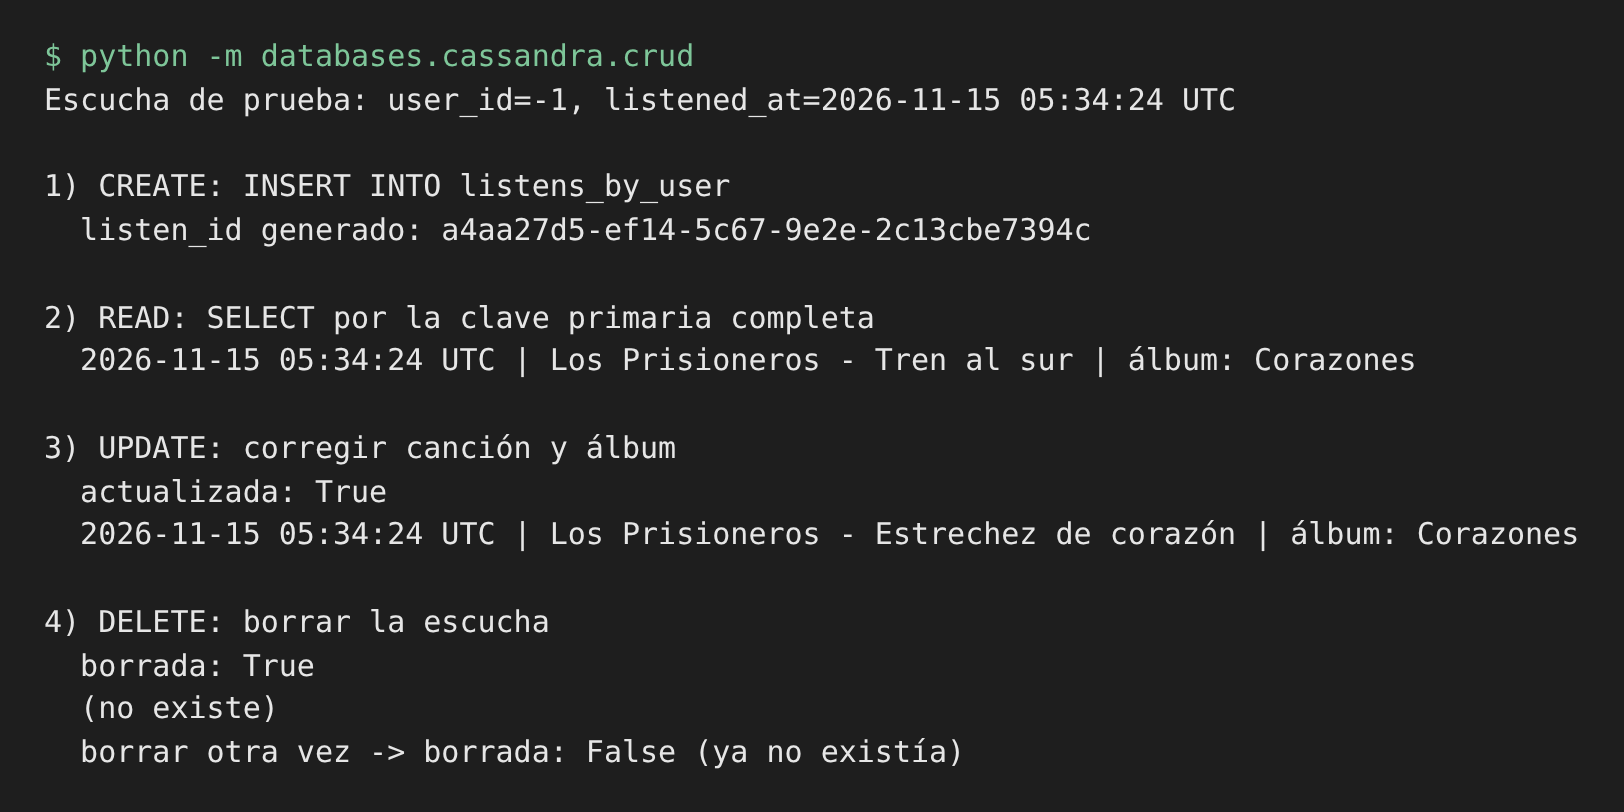
\includegraphics[width=0.9\textwidth]{figuras/cassandra_crud.png}
\nota{El quinto paso, la lectura de un usuario real, no se incluye para no publicar su identificador.}
\end{figure}

\subsection{Consultas}

\code{databases/cassandra/queries.py} tiene una función por consulta y todas devuelven listas de diccionarios, que el dashboard puede convertir directamente en tablas. Cada una lee una sola partición:

\begin{table}[H]
\centering
\caption{Consultas de Cassandra y tiempos medidos}
\label{tab:cassandra-consultas}
\begin{tabularx}{\textwidth}{l Y r}
\toprule
Función & Devuelve & Tiempo \\
\midrule
\code{get_daily_stats} & Escuchas, usuarios activos, escuchas por usuario y crecimiento de cada día del año & 6~ms \\
\code{get_top_artists} & Ranking del mes con escuchas y porcentaje del total & 11~ms \\
\code{get_artist_history} & Escuchas por mes de un artista & 16~ms \\
\code{get_user_activity} & Escuchas por día de un usuario & -- \\
\code{get_load_batches} & Lotes cargados, con filas cargadas y omitidas & -- \\
\bottomrule
\end{tabularx}
\nota{Tiempos medidos con el dataset completo: serie diaria de 2026, top 10 de octubre de 2026 e historial mensual de un artista. Leer las últimas 5 escuchas de la partición más grande de \code{listens_by_user} (14\,205 filas) tomó 14~ms.}
\end{table}

\subsection{Limitaciones}

El keyspace corre en un solo nodo con factor de replicación 1, que sirve para desarrollo pero no tolera caídas; en producción correspondería \code{NetworkTopologyStrategy} con factor 3. Los artistas se identifican por el nombre tal como viene en el dataset, así que homónimos y variantes de escritura cuentan por separado. Los agregados se recalculan desde el archivo, por lo que una escucha creada a mano con el CRUD no aparece en ellos. Por último, los duplicados se descartan dentro de cada lote; entre lotes \code{listens_by_user} no duplica (mismo id), pero los agregados contarían dos veces. En este dataset no hay duplicados: lo comprobamos sobre los 4\,855\,809 registros.
